\chapter{Magnetic Particle Imaging: Legacy Research Illustration}
\index{Magnetic Particle Imaging: Legacy Research Illustration}
\label{ch:infographic-mpi-legacy}
\begin{center}
  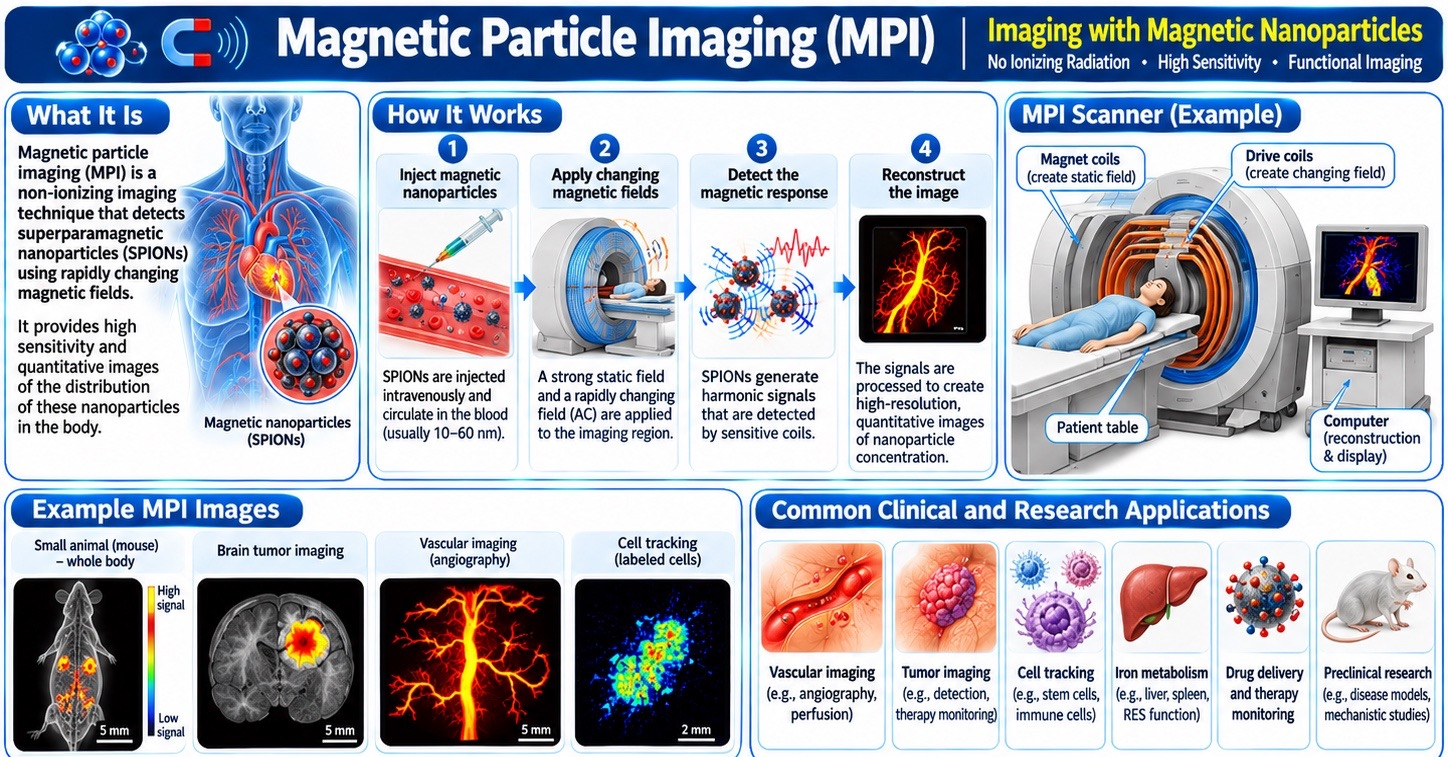
\includegraphics[width=\textwidth,height=0.6\textheight,keepaspectratio]{mpi.jpeg}
\end{center}
\noindent\textbf{Historical Context:} This earlier illustration is preserved for archival reference. It visually overstates clinical readiness---magnetic particle imaging (MPI) remains an investigational research modality with no FDA-approved clinical human scanner. For the current, medically vetted technical and safety summary of MPI, see Chapter~\ref{ch:infographic-mpi}.

\section{Why This Legacy Graphic Is Preserved}

Early promotional and conceptual illustrations of emerging medical technologies often depict compact, bedside, or routine hospital workflows long before full-scale human hardware, safety clearances, and approved tracers exist. Keeping this earlier MPI graphic alongside Chapter~\ref{ch:infographic-mpi} provides a concrete reminder of the gap between promising preclinical breakthroughs and routine clinical care.

\begin{itemize}
  \item \textbf{Current Clinical Status:} Invented in 2005, MPI has demonstrated impressive zero-background 3D tracking of superparamagnetic iron oxide nanoparticles (SPIONs) in small-animal scanners and early human-head research prototypes, but no clinical human MPI scanner is approved for routine diagnosis.
  \item \textbf{Key Translation Hurdles:} Scaling strong static magnetic gradients to full human-body size while staying within international peripheral nerve stimulation (PNS) and heating (SAR) limits, securing clinical approval for uniform MPI-optimized iron tracers, and pairing MPI with MRI or CT for anatomical context remain active areas of engineering research.
  \item \textbf{Standard Care Always Comes First:} Patients needing blood-vessel, stroke, bleeding, or cancer imaging today rely on established clinical modalities such as CT angiography (Chapter~\ref{ch:infographic-cta}), MRI/MRA (Chapters~\ref{ch:infographic-mri} and~\ref{ch:infographic-mra}), digital subtraction angiography (Chapter~\ref{ch:infographic-dsa}), or PET/CT (Chapter~\ref{ch:infographic-pet-ct}).
\end{itemize}

\section{Key References}
\begin{itemize}
  \item Gleich B, Weizenecker J. Tomographic imaging using the nonlinear response of magnetic particles. \textit{Nature}. 2005;435(7046):1214--1217.
  \item Graeser M, Thieben F, Szwargulski P, et al. Human-sized magnetic particle imaging for brain applications. \textit{Nature Communications}. 2019;10:1936.
  \item Talebloo N, Gudi M, Robertson N, Wang P. Magnetic particle imaging: current applications in biomedical research. \textit{Journal of Magnetic Resonance Imaging}. 2020;51(6):1659--1668.
  \item Harvell-Smith S, Tung LD, Thanh NTK. Magnetic particle imaging: tracer development and the biomedical applications of a radiation-free, sensitive, and quantitative imaging modality. \textit{Nanoscale} (NIH PubMed Central). 2022;14(10):3658--3697. Available at: \url{https://pmc.ncbi.nlm.nih.gov/articles/PMC8915192/}.
\end{itemize}

\section{Further Reading}
\begin{itemize}
  \item Wikipedia contributors. \textit{Magnetic particle imaging}. Wikipedia, The Free Encyclopedia. Available at: \url{https://en.wikipedia.org/wiki/Magnetic_particle_imaging}.
\end{itemize}
